\section{Developpement}

Maintenant que nous avons une analyse plus complète du domaine et plus particulièrement,  un arbre des features qui peuvent être intégrés dans le framework,  nous pouvons attaquer le développement.  Étant donné qu'il s'agit ici de programmation,  ce chapitre ne sera pas exhaustif du travail fourni mais permet de donner un aperçu de la façon de fonctionner.  Quelques exemples concrets et réels seront repris car nous éviterons de trainer sur des aspects trop techniques.  Nous allons commencer par décrire l'approche suivie pour la programmation du framework et ensuite,   nous passerons à la description du développement d'un feature choisi : la monnaie.  Celui-ci a été choisi car il permet de se rendre compte des différentes étapes pour l'implémentation d'un feature dans un projet Django.  Ce sera l'occasion de voir les techniques et patterns utilisés sans pour autant devoir expliquer trop de spécificités techniques liées à Django ou Python.  Notons que l'objectif ici est bien de modifier le code pour le rendre plus facile à appliquer par la suite.  Nous verrons dans le chapitre 7 (Validation) un exemple d'application concrète basée sur les features développés.   

\subsection{Approche}
Développer un framework est assez particulier et,  parce que nous partons d'un programme existant,  la méthode change quelques peu du cycle de développement habituel d'un logiciel.  Nous allons donc d'abord voir la façon dont nous allons fonctionner pour partir d'une solution existante spécifique et arriver à un framework plus générique,  dans le but de pouvoir ensuite dériver d'autres instances de ce framework.  Après avoir spécifié la méthode,  nous allons aborder rapidement un outil particulier qui a été utilisé pour le développement ainsi que les principales difficultés rencontrées pendant le processus.

\subsubsection{Développement d'un framework}

Le développement du framework va,  à l'instar de l'analyse,  se faire selon une démarche un peu particulière.  Pour illustrer celle-ci,  partons d'une comparaison.  Considérons qu'un logiciel est  comme un grand puzzle dont chaque pièce correspond à la partie du code liée à une fonctionnalité de l'application.  Dans le cas d'un framework,  le puzzle possède des trous à l'endroit de certaines pièces et c'est en complétant ces trous que l'on obtient une application fonctionnelle.  Pour pouvoir développer les features un à un,  la démarche utilisée consiste donc à d'abord tenter de retrouver,  dans le projet,  toutes les parties du code qui concernent le feature dont il est question pour ensuite reprogrammer cette partie pour qu'il soit plus facile d'adapter cette fonctionnalité selon les cas prévus.

Le schéma suivant reprend les principales étapes du développement.  D'abord,  nous avons un logiciel foncionnel.  Ensuite,  on identifie les parties de code liées aux fonctionnalités (1 pièce = 1 fonctionnalité).  Après cela,  il faut transformer ce code pour qu'i soit facilement adaptable selon la situation.  On obtient ainsi les pièces en bleu.  Et enfin,  lorsqu'on désire instancier notre framework à un cas particulier,  on pourra programmer dans les parties nécessaires,  qui correspondent aux pièces en vert.

\begin{center}
\fbox{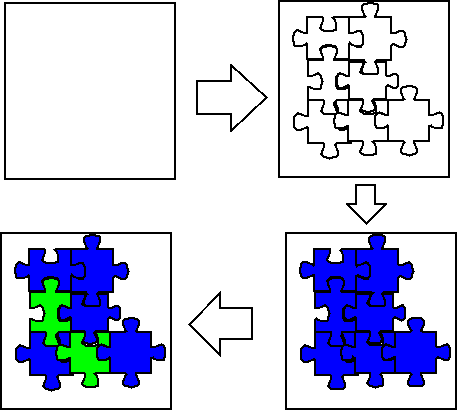
\includegraphics[scale=0.4]{puzzle.png}}
\end{center}

Enfin,  il est important de noter une difficulté particulière dans le cas du développement de notre framework.  En effet,  contrairement à une application orientée-objet classique,  notre framework est destiné au web.  Dès lors,  l'architecture est assez particulière et complique les choses pour toute la partie de retro-ingénierie du développement,  c'est-à-dire retrouver dans l'application,  les portions de code à traiter.  Cette complexité se rajoute aux diverses particularités de Django comme la description rigide du modèle de données ou les templates rédigés en HTML et quelques mots clés.

Pour faire face à cette complexité,  quelques outils peuvent aider lors du la rétro-ingénierie faite sur le logiciel de base (le travail du groupe 8) ainsi que pendant le développement.  Nous allons les décrire dans la prochaine section.

\subsubsection{Outils}

Pour nous aider dans le développement,  nous allons utiliser un simple script python récupéré d'internet et légèrement adapté.  Son principe est assez simple,  il parcourt toute l'arborescence du projet et ouvre les fichiers un par un.  Pour chacun d'eux,  il recherche le mot passé en argument du script.  Après chaque fichier,  si le script a trouvé au moins 1 occurence,  le nom et le chemin du fichier sont affichés dans la console avec le nombre d'occurences dans le fichier.  Ceci permet de rapidement retrouver quelles parties de code utilisent une classe ou fonction que l'on recherche,  à partir du mot clé donné.  Par exemple,  si nous voulons retrouver tous les endroits où l'attribut first\_name (d'un utilisateur) est utilisé,  il suffit de se placer à la racine du projet et de lancer la commande : python3 search.py first\_name.  Dans ce cas-ci,  pour l'exemple,  nous avons précisé qu'il ne fallait lire que les fichiers python (nomDuFichier.endswith(".py") ) et le résultat est : 

\begin{lstlisting}
Found matches:
/media/maxime/Data/framework/newTest/branch/tests.py ['first_name', 'first_name', ......... , 'first_name', 'first_name']
/media/maxime/Data/framework/newTest/branch/views.py ['first_name', 'first_name', 'first_name', 'first_name']
/media/maxime/Data/framework/newTest/care4care/adapter.py ['first_name', 'first_name', 'first_name']
/media/maxime/Data/framework/newTest/care4care/lookups.py ['first_name']
/media/maxime/Data/framework/newTest/main/admin.py ['first_name', 'first_name', 'first_name', 'first_name']
/media/maxime/Data/framework/newTest/main/forms.py ['first_name', 'first_name']
/media/maxime/Data/framework/newTest/main/models.py ['first_name', 'first_name', 'first_name', 'first_name', 'first_name', 'first_name']
/media/maxime/Data/framework/newTest/main/tests.py ['first_name', 'first_name', ......... ,  'first_name']
/media/maxime/Data/framework/newTest/main/test_statistics.py ['first_name', 'first_name']
/media/maxime/Data/framework/newTest/main/views.py ['first_name', 'first_name', 'first_name', 'first_name', 'first_name']
\end{lstlisting}

Grâce à cela,  nous savons quels sont les fichiers qui utilisent cet attribut.  Et si nous le modifions,  nous devons vérifier/modifier à chaque endroit le code correspondand. 

Une autre astuce a été utilisée pour pouvoir débugger dans Django pendant le développement.  Il s'agit d'une simple instruction python permettant d'insérer l'équivalent d'un breakpoint. 
\begin{lstlisting}
import pdb; pdb.set_trace()
\end{lstlisting}
Lorsque le serveur arrive à ce point d'arrêt,  il se met en pause et une console s'ouvre.  
Dans la console,  on peut inspecter toutes les variables du programme en cours.  C'est très utile pour vérifier que les données sont bien correctes entre différents appels/pages/requêtes.

\subsection{Recherche et implémentation des features}

Pour le développement du framework,  nous allons donc démarrer de l'application du groupe 8 et tenter d'y retrouver les portions de code qui sont liées à des features précis.  L'objectif sera donc de partir du fait que,  dans notre arbre des features,  le groupe 8 a mis en place un feature feuille,  et l'objectif va être de transformer le programme pour correspond à un branchement supérieur.

\subsubsection{Feature Temps}
Le premier feature que nous allons analyser consiste en la monnaie utilisée.  Le travail du groupe 8 a appliqué le feature "Temps -> Normal",  c'est à dire que la monnaie utilisée dans l'outil est du temps.  L'objectif de cette partie consiste donc à retrouver les parties du code liées à la monnaie et de trouver une solution pour rendre ces parties plus génériques.
\\
\textbf{main/models.py}
\\%=================
La première chose à retrouver dans le code se trouve dans la description du modèle.  On y retrouve la classe User avec un attribut Credit ainsi qu'une méthode permettant de traduire en mots la valeur du crédit.
\\
\textbf{main/forms.py}
\\%================
Un autre endroit concerné par le feature de la monnaie est le fichier forms.py,  toujours dans l'application main.  On y retrouve la classe GIftForm qui permet d'afficher le formulaire de don de temps à un utilisateur.  La valeur de credit apparait dans la méthode clean\_amount de cettte classe et est liée à la variable amount,  définie comme un champ de formulaire au début de la classe.
\\
\textbf{main/views.py}
\\%================
Dans ce fichier,  on retrouve les crédits dans la méthode destinée à générer la vue pour consulter la page contenant ses informations liées au crédit.  Celle-ci est accessible depuis le menu de gauche,  lorsqu'un utilisateur est connecté.  Le template associé se situe dans /main/templates/credit/ .
\\
\textbf{main/urls.py et main/urls\_credits.py}
\\%==================================
On retrouve ici d'abord le fichier des urls de l'application main qui inclus les urls liées aux crédits via le fichier urls\_credits.py.  Ce dernier contient simplement une url qui redirige vers la page décrite au point précédent.
\\
\textbf{main/templates/credit/credit\_page.html}
\\%=====================================
Ce template html permet d'afficher toutes les informations générées via les fichiers précédents.
\\
\textbf{branch/views.py}
\\%=================
Au sein de ce fichier,   on retrouve les crédits dans une méthode manage\_success.  Celle-ci clôture un échange fructueux et les crédits interviennent pour réaliser l'échange de monnaie.  
\\
\textbf{templates/base.html}
\\%=====================
Dans ce fichier,  on retrouve le message qui apaprait lorsqu'on est connecté et qui affiche le crédit restant.  Attention : l'élément CSS utilisé par cet affichage est aussi utilisé pour le type de compte.   
\\
\textbf{Divers fichiers de rendu visuel}
\\%============================
On notera enfin que quelques pages plus statiques liées à la couche vue (rendu graphique et traduction).  Par exemple,  les traductions se retrouvent dans les fichiers locale/*langue*/LC\_MESSAGES/django.po avec *langue* pouvant prendre les valeurs "en" et "nl".  Ensuite,  on retrouve aussi quelques propriétés CSS dans static/css/style.css 
\newline
Ceci clôture le côté utilisateurs des crédits.  Il reste à repérer l'utilisation de ceux-ci dans les transactions.  
\\
\textbf{branch/models.py}
\\%=================
Pour cela,  nous allons à nouveau rechercher les propriétés dans les descriptifs des modèles. 
On y retrouve la classe Demand,  qui hérite de la classe Job.  Dans Demand,  2 éléments nous concernent : estimated\_time et real\_time.  
Dans la classe Offer,  il n'y a pas d'éléments liés à la monnaie.  Ceci est lié à un choix de design de l'outil.  En effet,   lorsqu'on désire encoder une offre dans le système,  on doit préciser une date et un type de service à rendre mais pas de crédit.  Il n'y a donc pas de crédit pour une offre telle quelle.
\\
\textbf{branch/views.py}
\\%=================
Ensuite,  dans le fichier views.py du même dossier,   nous retrouvons 2 occurences de real\_time.  
Une première fois lors de l'assignation de la valeur de success.time à demand.real\_time.  Cela signifie que,  avant que la demande puisse être enregistrée pour l'historique,  on enregistre la valeur du temps réellement pris pour le service qui est validé,  c'est à dire l'instance success.
La seconde fois concerne le formulaire de création de demande.  On retrouve donc l'élément dans la classe CreateDemandView où real\_time reçoit la valeur qui avait été estimée à la base.  
\\
\textbf{main/views.py}
\\%================
Enfin dans ce fichier,  on retrouve l'élément real\_time mais dans une méthode qui a déjà été signalée précédemment puisqu'il s'agit de l'affichage des crédits.
\\
\textbf{main/ajax/views.py}
\\%====================
L'élément real\_time est aussi utilisé pour créer des statistiques qui seront exportées au format JSON.
\\
\textbf{branch/forms.py}
\\%=================
Dans ce fichier,   l'élément estimated\_time apparait plusieurs fois dans 3 méthodes de création de formulaire : l'enregistrement et l'édition d'une demande d'aide ainsi que la réponse à une offre d'aide.
\\
\textbf{Fichiers de rendu visuel}
\\%=======================
3 fichiers de templates sont concernés par l'élément estimated\_time dans le dossier branch/templates/job/ : details\_demand.html,  need\_help.html et take\_offer.html.

Maintenant que nous avons pu retrouver et comprendre les différentes portions de code qui sont impliquées dans le feature "Temps",  nous pouvons passer à l'action.  Pour ce faire,  allons suivre le cheminement général des appels dans l'application.  Mais juste avant,  précisons une dernière chose concernant la structure du logiciel dans lequel nous travaillons.  Il est important de rappeler que celle-ci est divisée en "sous-applications".  Chacune d'elle correspond à un sous-dossier du projet.  Les 2 sous-applications qui nous concernent sont Branch et Main.  Branch regroupe les fonctionnalités liées aux échanges et Main celles liées aux utilisateurs.  On remarque cette division en analysant le chemin des fichiers analysés ici avant (1 sous application = 1 sous-dossier).  

Les 2 types de points de départ que nous allons exploiter pour notre développement sont : les fichiers models.py qui définissent les modèles de données (1 par application),  et les templates,  qui contiennent des URL's qui représenteront les actions que les utilisateurs peuvent "activer".  

Pour le premier point qui concerne la description des modèles,  ce sont les fichiers models.py qui nous intéressent.  Dans l'analyse qui précède,  nous avions retrouvé 3 choses liées aux modèles : l'attribut Credit (et la fonction de type verbose qui va avec) dans la classe User,  définie dans l'application Main,  et les attributs estimated\_time et real\_time dans la classe Demand,  définie dans l'application Branch.  Le cas de la classe User est assez simple : nous allons simplement transformer la classe User ayant 1 attribut Crédit en 1 classe User qui peut hériter d'une autre classe,  qui elle-même possède l'attribut dont il est question.  Ceci permet de pouvoir hériter ou non de la classe (donc utilisation,  ou non,  d'une monnaie) ainsi que de définir dans une classe dédiée,  le comportement de la monnaie (dans le cas d'une monnaie alternative ou du temps ou autres).  

\begin{minipage}{.5\textwidth}
\begin{center} \textbf{Avant}\end{center}
\begin{lstlisting}
class User(AbstractBaseUser, PermissionsMixin, CommonInfo, VerifiedUser):
"""
Custom user class
"""
	email = models.EmailField(\_("Adresse email"), unique=False)
	...
	credit = models.IntegerField(default=0, verbose_name=\_("Credit restant")) # in minuts
	...
	def get_verbose_credit(self):
		credit = self.credit
		chunks = (...)
	...
	@models.permalink
	def get_absolute_url(self):
		return ('user_profile', (), {'user_id' : self.id})
\end{lstlisting} 
\end{minipage}
\hspace{0.3cm}
\begin{minipage}{.5\textwidth}
\begin{center} \textbf{Après}\end{center}
\begin{lstlisting}

class FWUser(models.Model):
    credit = models.IntegerField(default=0, verbose_name=_("Credit restant")) # in minuts   
    def get_verbose_credit(self):
        credit = self.credit
        chunks = (...)
        ...
    class Meta:
        abstract = True

class User(AbstractBaseUser, FWUser, PermissionsMixin, CommonInfo, VerifiedUser):
"""
Custom user class
"""
	...
\end{lstlisting} 
\end{minipage}


Le code décrivant le modèle pour les crédits des utilisateurs a ainsi été modifié pour être facilement adaptable selon le cadre dans lequel le logiciel sera utilisé.  Continuons donc notre cheminement à travers les appels dans l'application Django.  Nous allons faire la même chose pour les attributs liés aux demandes,  c'est-à-dire estimated\_time et real\_time dans branch/models.py.  

\begin{minipage}{.5\textwidth}
\begin{center} \textbf{Avant}\end{center}
\begin{lstlisting}
class Demand(Job):
    """ Representation of a demand """
    title = models.CharField( ...)
    ...
    estimated_time = models.IntegerField(verbose_name=_("Temps estime (en minutes)"), blank=True, null=True)
    real_time = models.IntegerField(verbose_name=_("Temps reel (en minutes)"), blank=True, null=True)
    ...
\end{lstlisting} 
\end{minipage}
\hspace{0.3cm}
\begin{minipage}{.5\textwidth}
\begin{center} \textbf{Après}\end{center}
\begin{lstlisting}
class FWMoney(models.Model):
    estimated_time = models.IntegerField(verbose_name=_("Temps estime (en minutes)"), blank=True, null=True)
    real_time = models.IntegerField(verbose_name=_("Temps reel (en minutes)"), blank=True, null=True)
    class Meta:
        abstract = True

class Demand(Job, FWMoney):
    """ Representation of a demand """
    title = models.CharField( ...)
    ...
\end{lstlisting} 
\end{minipage}


La description des classes liées à la base de données étant modifiée,  nous allons passer aux fichiers views.py,  qui correspondent à la couche Contrôlleur de l'application.  Selon l'analyse faite,  nous avons retrovué des utilisations des crédits,  entre autres,  pour l'affichage de la page décrivant les crédits de l'utilisateur,  lorsqu'il est connecté.  Cette même page permet également de faire un don de crédit à un autre utilisateur.  Pour l'affichage de formulaires,  le fichier views.py faire référence au fichier forms.py.  Ce dernier décrit les éléments de chaque formulaire et dans views.py,  nous importons ces descriptions et décrivons la logique derrière le formulaire.  Dès lors,  dans la sous-application Branch,  nous avons des crédits qui entrent en jeu (via les variable real et estimated\_time) dans la classe CreateDemandView(CreateView),  plus précisément dans la définition de la méthode : def form\_valid(self, form) ainsi que def manage\_success(request, success\_demand\_id).  La première classe est utilisé pour l'affichage du formulaire de crétaion d'une demande tandis que la seconde méthode,  elle,  est utilisée pour finaliser une transaction qui s'est déroulée avec succès.  Dans les 2 cas,  d'un point de vue technique,  la situation est différente de la modification des fichiers models.py.  En effet,  nous avons ici affaire à des descriptions de méthodes et il n'y a que quelques lignes de codes concernées par les crédits.  Etant donné que ces lignes en question sont des assignations de variable,  nous pouvons simplement décrire à chaque fois une méthode qui pourra être customisée et qui permettra de définir le comportement pour cette partie de l'application.  En concret,  voici quelques fragments de code pour mieux comprendre l'idée : 

\begin{minipage}{.5\textwidth}
\begin{center} \textbf{Avant}\end{center}
\begin{lstlisting}
class CreateDemandView(CreateView):
    def form_valid(self, form):
        ....
        form.instance.receiver = User.objects.get(pk=self.kwargs['user_id'])
        form.instance.real_time = form.instance.estimated_time
        return super(CreateDemandView, self).form_valid(form)

def manage_success(request, success_demand_id):
	...
          demand.real_time =  success.time
          demand.success = True
          demand.donor.credit += success.time
          demand.donor.save()
          demand.receiver.credit -= success.time
          demand.receiver.save()
\end{lstlisting} 
\end{minipage}
\hspace{0.3cm}
\begin{minipage}{.5\textwidth}
\begin{center} \textbf{Après}\end{center}
\begin{lstlisting}

def fw_man_success(demand, successTime):
    if successTime > 100000:
        successTime = 100000
    if successTime < 0:
        successTime = 0
    demand.real_time =  successTime
    demand.donor.credit += successTime
    demand.receiver.credit -= successTime  
    return demand

def fw_form_valid(form):
    form.instance.real_time = form.instance.estimated_time
    return form
...
...
class CreateDemandView(CreateView):
    def form_valid(self, form):
        ....
        form = fw_form_valid(form)
...
def manage_success(request, success_demand_id):
	...
         demand = fw_man_success(demand,  success.time)
...
\end{lstlisting} 
\end{minipage}

Concernant le fichier views.py de la sous-application Main (qui gère donc les utilisateurs),  nous retrouvons une seule méthode permettant d'afficher la page des crédits.  Étant donné que l'entièreté de la méthode est dédiée au feature temps,  il suffit d'isoler celle-ci pour la rendre plus accessible en cas de modification.  Pour cela,  nous avons simplement créé un fichier reprenant le code lié au framework.  Chaque fichier "couche" (models.py,  views.py,  forms.py) a donc un homonyme fw\_models.py,  fw\_views.py ,  etc .  Chacun de ces fichiers reprend les classes et méthodes adaptées dans le cadre du framework.  Cest le cas de la méthode def credits\_view(request) qui se retrouve entièrement dans le fichier "annexe".  Notons qu'il n'est pas toujours possible d'isoler les éléments dans un fichier séparé.  Reprenons l'exemple de models.py.  Dans ce cas là,  models.py importe les méthodes de fw\_models.py.  Mais fw\_models.py peut avoir besoin de la description de certains éléments de models.py.  Nous avons donc une boucle d'inclusion.  Ce qui implique que tout le code n'est pas systématiquement isolé dans un fichier différent.  

Pour la suite du développement,  nous allons suivre le second point de départ qui est donc les URL's.  Pour cela,  nous pouvons modifier les fichiers urls.py.  Il s'agit simplement,  pour chaque application,  de la liste des URL's prises en charges ainsi que la méthode ou la classe qui y est liée.  Pour la sous-application Branch,  il n'y a pas de référence directe au feature temps car les adresses gèrent les transactions.  Par contre,  dans la sous-application Main,  nous avons un fichier urls\_credits.py qui est inclus dans le fichier principal urls.py.  Ce fichier décrit une URL permettant d'accéder à la page d'affichage de crédits,  et fait référence à la méthode credits\_view,  que nous avons isolé précédemment.  Ainsi,  si vous voulons supprimer l'utilisation d'une monnaie dans le système,  cette référenc e peut être supprimée.  

Les derniers éléments à modifier pour mettre en place notre feature concernent la couche de vue de l'application.  Pour cela,  nous devons modifier les templates utilisés. Le premier est base.html.  Celui-ci,  comme son nom l'indique,  est le cannevas de base de toutes les pages de l'application.  C'est ce template qui permet,  par exemple,  d'afficher le menu supérieur et latéral gauche.  On y retrouve d'ailleurs l'affichage des crédits accumulés par l'utilisateur.  Cette référence doit être supprimée si on ne ddésire pas utliser de monnaie,  par exemple.  Pour faciliter l'adaptation,  nous allons isoler le code lié à cet affichage dans un "sous-template" auquel nous ferons appel dans base.html.  La même technique est utilisée pour le lien "Mes crédits" dans le menu latéral gauche.  Ci-dessous,  l'exemple illustré.  Ces fragments de code montrent comment ne pas afficher de crédits,  dans le cas d'une absence du feature monnaie,  donc.  

\begin{minipage}{.5\textwidth}
\begin{center} \textbf{Avant}\end{center}
\begin{lstlisting}
...
<p class="centered credit-p"><span class="credit-text"></span> {{ request.user.get_verbose_credit | safe }}</p>
...

<ul class="sub">
<li><span><a href=""> </a></span></li>
</ul>

...
\end{lstlisting} 
\end{minipage}
\hspace{0.3cm}
\begin{minipage}{.5\textwidth}
\begin{center} \textbf{Après}\end{center}
\begin{lstlisting}
...

...

...

Dans fw_base.html : 
<!--

<p class="centered credit-p"><span class="credit-text"></span> {{ request.user.get_verbose_credit | safe }}</p>

-->

Dans fw_base2.html : 
<!--

<ul class="sub">
     <li><span><a href=""> </a></span></li>
                </ul>

-->
\end{lstlisting} 
\end{minipage}




\subsection{Architecture du framework}

TO DO


